\section{Implementarea DVM versiunea 1}

Primul pas al implementării a fost reprezentat de alegerea modelelor \gls{yang} care să fie expuse de serverul \gls{netconf}. În cea de-a doua demonstraţie de concept \gls{wt} a fost agreată folosirea unor modele informaționale reduse, care să permită demonstrarea cazurilor de utilizare alese \cite{onf2016_poc2}. Acestea conţineau aproximativ şaizeci de atribute care făceau parte atât din modelul informațional de bază, cât și din modelul informațional pentru microunde. Astfel, au fost alese trei modele \gls{yang} pentru implementarea în cadrul primei versiuni a \gls{dvm}: \textit{CoreModel-CoreNetworkModule-ObjectClasses}, \textit{MicrowaveModel-ObjectClasses-MwConnection} și \textit{MicrowaveModel-Notifications}. Asta a însemnat, practic, generarea a trei biblioteci partajate reprezentând module ale serverului \gls{netconf}, care să poată fi încărcate în soluţia \textit{OpenYuma} și să ofere capabilitățile dorite.

O organigramă a fazei de dezvoltare și implementare a \gls{dvm} este ilustrată în Figura \ref{fig:dvm_v01_workflow}.

\begin{figure}[h]
	\centering
	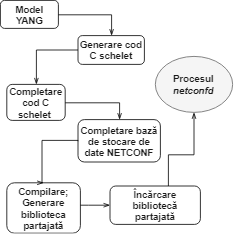
\includegraphics{dvm_v01_workflow}
	\caption{Organigramă a dezvoltării și implementării DVM \cite{stancu2016default}.}
	\label{fig:dvm_v01_workflow}
\end{figure}

Cel de-al doilea pas al implementării a constat în procesarea modelelor \gls{yang} alese și generarea codului C schelet al modulelor asociate acestora. Acest lucru a fost realizat cu utilitarul \textit{yangdump} oferit de soluţia \textit{OpenYuma}. Pentru a îmbunătăţi flexibilitatea \gls{dvm} și pentru a avea o mai bună separare între codul folosit de server și codul utilizatorului, care trebuie rescris, utilitarul a fost folosit cu opţiunea \textit{--split}. Astfel, pentru fiecare modul au fost generate patru fişiere: câte unul \textit{.c} și \textit{.h} pentru codul de server, respectiv pentru cel de utilizator.

Următorul pas a fost reprezentat de implementarea funcţiilor cu apel invers generate pentru fiecare atribut al modelului \gls{yang}. Pentru a asocia câte o valoare implicită fiecărui parametru, funcțiile au fost modificate astfel încât să întoarcă valoarea respectivă în momentul apelării.

Cea mai importantă parte a implementării \gls{dvm} a constat în construirea bazei de stocare a datelor de operare, reprezentând de fapt arborele atributelor \gls{yang} pe care serverul \gls{netconf} le va utiliza atunci când va fi interogat de către echipamentul de control \gls{sdn}. Nu a fost posibilă construirea automată a acestui arbore de parametri, astfel că atributele au fost implementate manual, de la rădăcină către frunze. Pentru acest lucru a fost nevoie să se altereze funcţia de iniţializare \textit{init2()} generată automat pentru fiecare model \gls{yang}. A fost necesară adăugarea câte unui nod \textit{OpenYuma} pentru fiecare parametru \gls{yang}, având asociată o funcție cu apel invers în care se setează valoarea implicită a acelui atribut. În cazul parametrilor anterior menţionaţi, care fac parte din fişierul de configurare, implementarea funcţiei constă în citirea valorii respective din acel fişier. Această abordare a permis utilizatorilor \gls{dvm} un acces facil la valorile implicite asociate fiecărui atribut. Dacă un utilizator avea nevoie de schimbarea valorii unui parametru \gls{yang}, o putea face uşor prin funcţia cu apel invers asociată sau prin fişierul de configurare, fără să fie nevoit să ştie detaliile de implementare referitoare la construirea arborelui de valori.

Următorii paşi ai implementării sunt simpli și direcţi: codul rezultat se compilează, rezultând bibliotecile partajate care apoi sunt încărcate în serverul \gls{netconf} (mai exact în procesul \textit{netconfd} asociat acestuia).

Etapele anterior menţionate se aplică în cazul modelului informațional de bază și în cazul modelului informațional pentru microunde, excluzând cazul notificărilor \gls{netconf}, unde abordarea este puţin diferită.

Deoarece modelul asociat notificărilor \gls{netconf}, \textit{MicrowaveModel-Notifications}, are o structură diferită, conţinând obiecte \gls{yang} ce reprezintă notificări în locul atributelor obişnuite, comportamentul soluţiei \textit{OpenYuma} este diferit în acest caz. În loc să se genereze funcții cu apel invers pentru obţinerea și setarea valorilor atributelor, în cazul notificărilor soluţia \textit{OpenYuma} va genera funcții cu apel invers folosite pentru declanşarea acestora (trimiterea lor de către server tuturor utilizatorilor care s-au abonat).

Pentru implementarea notificărilor \gls{netconf} în \gls{dvm}, un nou fir de execuţie s-a creat în funcţia de iniţializare a modulului, \textit{init2()}. Acesta rulează o singură funcție care implementează o buclă infinită în care se folosește funcţia cu apel invers asociată pentru a trimite o notificare fictivă, la un interval de secunde definit în fişierul de configurare. În cazul în care valoarea intervalului este zero, declanşarea notificărilor nu va fi activată. Detaliile conţinute în notificarea \gls{netconf} fictivă se găsesc în interiorul funcţiei care implementează generarea și modificarea acestora nu este banală pentru un utilizator neexperimentat.

Structura fişierului de configurare este foarte simplă și nu oferă prea multă flexibilitate utilizatorilor \gls{dvm}. Aceasta este fixă și poate fi observată în Figura \ref{fig:dvm_v01_config}, într-un exemplu în care un dispozitiv conţine două interfețe radio. Conţine doar trei tipuri de parametri, așa cum a fost menţionat anterior: numele echipamentului de rețea (\textit{NeName}), identificatoarele legăturilor radio (\textit{radioSignalId} - există câte un identificator pentru fiecare interfață radio a dispozitivului) și intervalul de timp, exprimat în secunde, dintre două notificări fictive consecutive (\textit{eventFrequency}).

\begin{figure}[h]
	\centering
	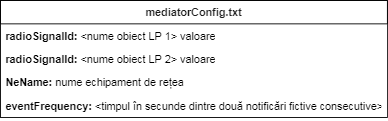
\includegraphics{dvm_v01_config}
	\caption{Structura fişierului de configurare al DVM. Exemplu pentru un echipament cu două interfețe radio.}
	\label{fig:dvm_v01_config}
\end{figure}